% Chapter in which we explore how well various approaches do.

\chapter{Results}
\label{ch:results}

In this chapter, we compare the various alternatives discussed in Chapter
\ref{ch:methods}. We test each of the alternatives on the randomly generated
dataset
containing \q test schematics. All of the alternatives are evaluated on this
same dataset for appropriate comparison.

To assess the goodness of an alternative method, we give:
\begin{enumerate}
\item A diagram of a 2D array of points in which each point represents a run.
Each point is colored white or red corresponding to a successful or unsuccessful
run, respectively. This array gives a general overview of how well the method
performed on the test dataset.
\item The success rate of the method on the test dataset. The higher this value,
the better the method.
\item The average and standard deviation of success times. The lower the average,
the better the method.
\item The average and standard deviation of failure times. The lower the average,
the better the method.
\item Among the solved schematics, the average and standard deviation of the
number of wires used. The lower the average, the better the method.
\item Among the solved schematics, the average and standard deviation of the
total wire length of the wires on the protoboard. The lower the average, the
better the method.
\item Among the solved schematics, the average and standard deviation of the
number of wire crosses on the protoboard. The lower the average, the better the
method.
\end{enumerate}

To assess the effect of various aspects of schematics on the method, we give
tables in which we consider the values of each of the following items, and
record how success rate, average success time, and average failure time depend
on the values:
\begin{enumerate}
\item Number of components.
\item Number of nodes in the circuit.
\item Number of resistors.
\item Number of Op Amps.
\item Number of pots.
\item Number of motors.
\item Number of Head Connectors ($0$ or $1$).
\item Number of Robot Connectors ($0$ or $1$).
\end{enumerate}

Analysis of the results follows in Chapter \ref{ch:discussion}.

\section{Resistors as Components}

First we consider the case in which we treat resistors as components. That is,
the resistors in the circuit will be placed on the protoboard by the placement
step. With this setup, we consider $5$ different ways of wiring.

\subsection{All connections at once}

Here we consider connecting all pairs of location that need to
be connected at once. Figure \ref{fig:as_comp_all} displays the overall results.
Table \ref{tb:as_comp_all} presents the statistics we obtain with this setup.

\begin{figure}[H]
\begin{center}

\includegraphics{Images/placeholder.jpg}
\caption{Overall results when we treat resistors as components and connect all
pairs of protoboard locations at once.}
\label{fig:as_comp_all}
\end{center}
\end{figure}

\begin{table}[H]
\begin{center}
\begin{singlespace}
\begin{tabular}{| c | c |}
\hline
Item & Value \\
\hline\hline
Success rate & \\
Solve time mean and standard deviation & \\
Failure time mean and standard deviation & \\
Number of wires mean and standard deviation & \\
Total wire length mean and standard deviation & \\
Total wire crosses mean and standard deviation & \\
\hline
\end{tabular}
\end{singlespace}
\end{center}
\label{tb:as_comp_all}
\caption{Test statistics when we treat resistors as components and connect all
pairs of protoboard locations at once.}
\end{table}

\subsection{Connections for one node at a time, node with \textit{most}
connections first}

Next we consider connecting the location pairs for one node at a time, ordered
in \textit{descending} order of number of location pairs per node. Figure
\ref{fig:as_comp_node_d} shows the overall results, and Table
\ref{tb:as_comp_node_d} presents the statistics for this setup.

\begin{figure}[H]
\begin{center}

\includegraphics{Images/placeholder.jpg}
\caption{Overall results when we treat resistors as components and connect the
location pairs for one node at a time, with the node with the most connections
going first.}
\label{fig:as_comp_node_d}
\end{center}
\end{figure}

\begin{table}[H]
\begin{center}
\begin{singlespace}
\begin{tabular}{| c | c |}
\hline
Item & Value \\
\hline\hline
Success rate & \\
Solve time mean and standard deviation & \\
Failure time mean and standard deviation & \\
Number of wires mean and standard deviation & \\
Total wire length mean and standard deviation & \\
Total wire crosses mean and standard deviation & \\
\hline
\end{tabular}
\end{singlespace}
\end{center}
\label{tb:as_comp_node_d}
\caption{Test statistics when we treat resistors as components and connect the
location pairs one node at a time, with the node with the most connections going
first.}
\end{table}

\subsection{Connections for one node at a time, node with \textit{least}
connections first}

Here also, we consider connecting the location pairs for one node at a time,
but this time ordered in \textit{ascending} order of number of location pairs
per node. Figure \ref{fig:as_comp_node_a} shows the overall results, and Table
\ref{tb:as_comp_node_a} presents the statistics for this setup.

\begin{figure}[H]
\begin{center}

\includegraphics{Images/placeholder.jpg}
\caption{Overall results when we treat resistors as components and connect the
location pairs for one node at a time, with the node with the least connections
going first.}
\label{fig:as_comp_node_a}
\end{center}
\end{figure}

\begin{table}[H]
\begin{center}
\begin{singlespace}
\begin{tabular}{| c | c |}
\hline
Item & Value \\
\hline\hline
Success rate & \\
Solve time mean and standard deviation & \\
Failure time mean and standard deviation & \\
Number of wires mean and standard deviation & \\
Total wire length mean and standard deviation & \\
Total wire crosses mean and standard deviation & \\
\hline
\end{tabular}
\end{singlespace}
\end{center}
\label{tb:as_comp_node_a}
\caption{Test statistics when we treat resistors as components and connect the
location pairs one node at a time, with the node with the least connections
going first.}
\end{table}

\subsection{One connection at a time, \textit{shortest} connection first}

Now we look at wiring one pair of locations at a time. First, we consider
starting from the closest pair of locations. Figure \ref{fig:as_comp_pair_s}
shows the overall results and Table \ref{tb:as_comp_pair_s} presents the
statistics for this setup.

\begin{figure}[H]
\begin{center}

\includegraphics{Images/placeholder.jpg}
\caption{Overall results when we treat resistors as components and connect one
pair of locations at a time, starting with the closest pair of locations.}
\label{fig:as_comp_pair_s}
\end{center}
\end{figure}

\begin{table}[H]
\begin{center}
\begin{singlespace}
\begin{tabular}{| c | c |}
\hline
Item & Value \\
\hline\hline
Success rate & \\
Solve time mean and standard deviation & \\
Failure time mean and standard deviation & \\
Number of wires mean and standard deviation & \\
Total wire length mean and standard deviation & \\
Total wire crosses mean and standard deviation & \\
\hline
\end{tabular}
\end{singlespace}
\end{center}
\label{tb:as_comp_pair_s}
\caption{Test statistics when we treat resistors as components and connect one
pair of locations at a time, starting with the closest pair of locations.}
\end{table}

\subsection{One connection at a time, \textit{longest} connection first}

Here we connect one pair of locations a time, but this time we start with the
farthest pair of locations. Figure \ref{fig:as_comp_pair_l} shows the overall
results and Table \ref{tb:as_comp_pair_l} presents the statistics for this
setup.

\begin{figure}[H]
\begin{center}
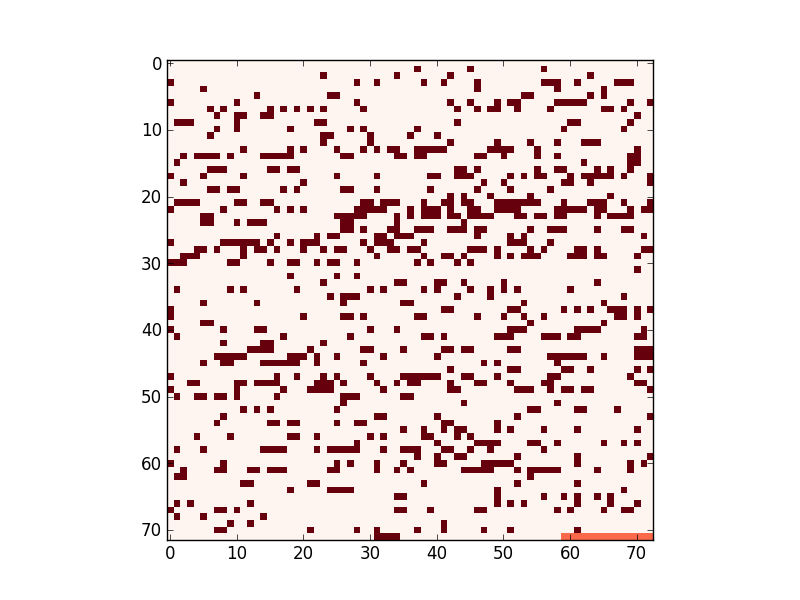
\includegraphics[width=\textwidth]{Images/overview_sample.png}
\caption{Overall results when we treat resistors as components and connect one
pair of locations at a time, starting with the farthest pair of locations.}
\label{fig:as_comp_pair_l}
\end{center}
\end{figure}

\begin{table}[H]
\begin{center}
\begin{singlespace}
\begin{tabular}{| c | c |}
\hline
Item & Value \\
\hline\hline
Success rate & \\
Solve time mean and standard deviation & \\
Failure time mean and standard deviation & \\
Number of wires mean and standard deviation & \\
Total wire length mean and standard deviation & \\
Total wire crosses mean and standard deviation & \\
\hline
\end{tabular}
\end{singlespace}
\end{center}
\label{tb:as_comp_pair_l}
\caption{Test statistics when we treat resistors as components and connect one
pair of locations at a time, starting with the farthest pair of locations.}
\end{table}

\subsection{Choice}

With resistors being treated as components, the test results suggest that the
best way to wire the components is \q. Next we look at the effects of various
aspects of the schematics on this method.

\begin{table}[H]
\begin{center}
\begin{singlespace}
\begin{tabular}{| c | c | c | c | c |}
\hline
Nodes & Sample size & Success rate & Success time mean & Failure time mean\\
\hline\hline
0 & & & & \\
1 & & & & \\
2 & & & & \\
3 & & & & \\
4 & & & & \\
5 & & & & \\
6 & & & & \\
7 & & & & \\
8 & & & & \\
9 & & & & \\
10 & & & & \\
\hline
\end{tabular}
\end{singlespace}
\end{center}
\label{tb:TODO}
\caption{TODO}
\end{table}

\begin{table}[H]
\begin{center}
\begin{singlespace}
\begin{tabular}{| c | c | c | c | c |}
\hline
Components & Sample size & Success rate & Success time mean & Failure time mean\\
\hline\hline
0 & & & & \\
1 & & & & \\
2 & & & & \\
3 & & & & \\
4 & & & & \\
5 & & & & \\
6 & & & & \\
7 & & & & \\
8 & & & & \\
9 & & & & \\
10 & & & & \\
11 & & & & \\
12 & & & & \\
13 & & & & \\
14 & & & & \\
15 & & & & \\
16 & & & & \\
17 & & & & \\
18 & & & & \\
\hline
\end{tabular}
\end{singlespace}
\end{center}
\label{tb:TODO}
\caption{TODO}
\end{table}

\begin{table}[H]
\begin{center}
\begin{singlespace}
\begin{tabular}{| c | c | c | c | c |}
\hline
Resistors & Sample size & Success rate & Success time mean & Failure time mean\\
\hline\hline
0 & & & & \\
1 & & & & \\
2 & & & & \\
3 & & & & \\
4 & & & & \\
5 & & & & \\
6 & & & & \\
7 & & & & \\
8 & & & & \\
9 & & & & \\
10 & & & & \\
11 & & & & \\
12 & & & & \\
13 & & & & \\
14 & & & & \\
15 & & & & \\
16 & & & & \\
17 & & & & \\
18 & & & & \\
\hline
\end{tabular}
\end{singlespace}
\end{center}
\label{tb:TODO}
\caption{TODO}
\end{table}

\begin{table}[H]
\begin{center}
\begin{singlespace}
\begin{tabular}{| c | c | c | c | c |}
\hline
Op Amps & Sample size & Success rate & Success time mean & Failure time mean\\
\hline\hline
0 & & & & \\
1 & & & & \\
2 & & & & \\
3 & & & & \\
4 & & & & \\
5 & & & & \\
6 & & & & \\
\hline
\end{tabular}
\end{singlespace}
\end{center}
\label{tb:TODO}
\caption{TODO}
\end{table}

\begin{table}[H]
\begin{center}
\begin{singlespace}
\begin{tabular}{| c | c | c | c | c |}
\hline
Pots & Sample size & Success rate & Success time mean & Failure time mean\\
\hline\hline
0 & & & & \\
1 & & & & \\
2 & & & & \\
3 & & & & \\
4 & & & & \\
5 & & & & \\
6 & & & & \\
\hline
\end{tabular}
\end{singlespace}
\end{center}
\label{tb:TODO}
\caption{TODO}
\end{table}

\begin{table}[H]
\begin{center}
\begin{singlespace}
\begin{tabular}{| c | c | c | c | c |}
\hline
Motors & Sample size & Success rate & Success time mean & Failure time mean\\
\hline\hline
0 & & & & \\
1 & & & & \\
2 & & & & \\
3 & & & & \\
4 & & & & \\
5 & & & & \\
6 & & & & \\
\hline
\end{tabular}
\end{singlespace}
\end{center}
\label{tb:TODO}
\caption{TODO}
\end{table}

\begin{table}[H]
\begin{center}
\begin{singlespace}
\begin{tabular}{| c | c | c | c | c |}
\hline
Head Connectors & Sample size & Success rate & Success time mean &
Failure time mean\\
\hline\hline
0 & & & & \\
1 & & & & \\
\hline
\end{tabular}
\end{singlespace}
\end{center}
\label{tb:TODO}
\caption{TODO}
\end{table}

\begin{table}[H]
\begin{center}
\begin{singlespace}
\begin{tabular}{| c | c | c | c | c |}
\hline
Robot Connectors & Sample size & Success rate & Success time mean &
Failure time mean\\
\hline\hline
0 & & & & \\
1 & & & & \\
\hline
\end{tabular}
\end{singlespace}
\end{center}
\label{tb:TODO}
\caption{TODO}
\end{table}

\section{Resistors as Wires}

Now we consider the case in which we treat resistors as wires. That is, the
resistors in the circuit will not be placed on the protoboard by the placement
step. Rather, we will place them in the wiring process as described in Section
\ref{sec:resistors_as_wires}. With this setup, we consider the $5$ different
ways of wiring once more.

\subsection{All connections at once}

Figure \ref{fig:as_wire_all} displays the overall results and Table
\ref{tb:as_wire_all} presents the statistics we obtain with this setup.

\begin{figure}[H]
\begin{center}

\includegraphics{Images/placeholder.jpg}
\caption{Overall results when we treat resistors as wires and connect all
pairs of protoboard locations at once.}
\label{fig:as_wire_all}
\end{center}
\end{figure}

\begin{table}[H]
\begin{center}
\begin{singlespace}
\begin{tabular}{| c | c |}
\hline
Item & Value \\
\hline\hline
Success rate & \\
Solve time mean and standard deviation & \\
Failure time mean and standard deviation & \\
Number of wires mean and standard deviation & \\
Total wire length mean and standard deviation & \\
Total wire crosses mean and standard deviation & \\
\hline
\end{tabular}
\end{singlespace}
\end{center}
\label{tb:as_wire_all}
\caption{Test statistics when we treat resistors as wires and connect all
pairs of protoboard locations at once.}
\end{table}

\subsection{Connections for one node at a time, node with \textit{most}
connections first}

Figure \ref{fig:as_wire_node_d} shows the overall results, and Table
\ref{tb:as_wire_node_d} presents the statistics for this setup.

\begin{figure}[H]
\begin{center}

\includegraphics{Images/placeholder.jpg}
\caption{Overall results when we treat resistors as wires and connect the
location pairs for one node at a time, with the node with the most connections
going first.}
\label{fig:as_wire_node_d}
\end{center}
\end{figure}

\begin{table}[H]
\begin{center}
\begin{singlespace}
\begin{tabular}{| c | c |}
\hline
Item & Value \\
\hline\hline
Success rate & \\
Solve time mean and standard deviation & \\
Failure time mean and standard deviation & \\
Number of wires mean and standard deviation & \\
Total wire length mean and standard deviation & \\
Total wire crosses mean and standard deviation & \\
\hline
\end{tabular}
\end{singlespace}
\end{center}
\label{tb:as_wire_node_d}
\caption{Test statistics when we treat resistors as wires and connect the
location pairs one node at a time, with the node with the most connections going
first.}
\end{table}

\subsection{Connections for one node at a time, node with \textit{least}
connections first}

Figure \ref{fig:as_wire_node_a} shows the overall results, and Table
\ref{tb:as_wire_node_a} presents the statistics for this setup.

\begin{figure}[H]
\begin{center}

\includegraphics{Images/placeholder.jpg}
\caption{Overall results when we treat resistors as wires and connect the
location pairs for one node at a time, with the node with the least connections
going first.}
\label{fig:as_wire_node_a}
\end{center}
\end{figure}

\begin{table}[H]
\begin{center}
\begin{singlespace}
\begin{tabular}{| c | c |}
\hline
Item & Value \\
\hline\hline
Success rate & \\
Solve time mean and standard deviation & \\
Failure time mean and standard deviation & \\
Number of wires mean and standard deviation & \\
Total wire length mean and standard deviation & \\
Total wire crosses mean and standard deviation & \\
\hline
\end{tabular}
\end{singlespace}
\end{center}
\label{tb:as_wire_node_a}
\caption{Test statistics when we treat resistors as wires and connect the
location pairs one node at a time, with the node with the least connections
going first.}
\end{table}

\subsection{One connection at a time, \textit{shortest} connection first}

Figure \ref{fig:as_wire_pair_s}
shows the overall results and Table \ref{tb:as_wire_pair_s} presents the
statistics for this setup.

\begin{figure}[H]
\begin{center}

\includegraphics{Images/placeholder.jpg}
\caption{Overall results when we treat resistors as wires and connect one
pair of locations at a time, starting with the closest pair of locations.}
\label{fig:as_wire_pair_s}
\end{center}
\end{figure}

\begin{table}[H]
\begin{center}
\begin{singlespace}
\begin{tabular}{| c | c |}
\hline
Item & Value \\
\hline\hline
Success rate & \\
Solve time mean and standard deviation & \\
Failure time mean and standard deviation & \\
Number of wires mean and standard deviation & \\
Total wire length mean and standard deviation & \\
Total wire crosses mean and standard deviation & \\
\hline
\end{tabular}
\end{singlespace}
\end{center}
\label{tb:as_wire_pair_s}
\caption{Test statistics when we treat resistors as wires and connect one
pair of locations at a time, starting with the closest pair of locations.}
\end{table}

\subsection{One connection at a time, \textit{longest} connection first}

Figure \ref{fig:as_wire_pair_l} shows the overall
results and Table \ref{tb:as_wire_pair_l} presents the statistics for this
setup.

\begin{figure}[H]
\begin{center}

\includegraphics{Images/placeholder.jpg}
\caption{Overall results when we treat resistors as wires and connect one
pair of locations at a time, starting with the farthest pair of locations.}
\label{fig:as_wire_pair_l}
\end{center}
\end{figure}

\begin{table}[H]
\begin{center}
\begin{singlespace}
\begin{tabular}{| c | c |}
\hline
Item & Value \\
\hline\hline
Success rate & \\
Solve time mean and standard deviation & \\
Failure time mean and standard deviation & \\
Number of wires mean and standard deviation & \\
Total wire length mean and standard deviation & \\
Total wire crosses mean and standard deviation & \\
\hline
\end{tabular}
\end{singlespace}
\end{center}
\label{tb:as_wire_pair_l}
\caption{Test statistics when we treat resistors as wires and connect one
pair of locations at a time, starting with the farthest pair of locations.}
\end{table}

\subsection{Choice}

With resistors being treated as wires, the test results suggest that the best
way to wire the components is \q. Next we look at the effects of various aspects
of the schematics on this method.

\begin{table}[H]
\begin{center}
\begin{singlespace}
\begin{tabular}{| c | c | c | c | c |}
\hline
Nodes & Sample size & Success rate & Success time mean & Failure time mean\\
\hline\hline
0 & & & & \\
1 & & & & \\
2 & & & & \\
3 & & & & \\
4 & & & & \\
5 & & & & \\
6 & & & & \\
7 & & & & \\
8 & & & & \\
9 & & & & \\
10 & & & & \\
\hline
\end{tabular}
\end{singlespace}
\end{center}
\label{tb:TODO}
\caption{TODO}
\end{table}

\begin{table}[H]
\begin{center}
\begin{singlespace}
\begin{tabular}{| c | c | c | c | c |}
\hline
Components & Sample size & Success rate & Success time mean & Failure time mean\\
\hline\hline
0 & & & & \\
1 & & & & \\
2 & & & & \\
3 & & & & \\
4 & & & & \\
5 & & & & \\
6 & & & & \\
7 & & & & \\
8 & & & & \\
9 & & & & \\
10 & & & & \\
11 & & & & \\
12 & & & & \\
13 & & & & \\
14 & & & & \\
15 & & & & \\
16 & & & & \\
17 & & & & \\
18 & & & & \\
\hline
\end{tabular}
\end{singlespace}
\end{center}
\label{tb:TODO}
\caption{TODO}
\end{table}

\begin{table}[H]
\begin{center}
\begin{singlespace}
\begin{tabular}{| c | c | c | c | c |}
\hline
Resistors & Sample size & Success rate & Success time mean & Failure time mean\\
\hline\hline
0 & & & & \\
1 & & & & \\
2 & & & & \\
3 & & & & \\
4 & & & & \\
5 & & & & \\
6 & & & & \\
7 & & & & \\
8 & & & & \\
9 & & & & \\
10 & & & & \\
11 & & & & \\
12 & & & & \\
13 & & & & \\
14 & & & & \\
15 & & & & \\
16 & & & & \\
17 & & & & \\
18 & & & & \\
\hline
\end{tabular}
\end{singlespace}
\end{center}
\label{tb:TODO}
\caption{TODO}
\end{table}

\begin{table}[H]
\begin{center}
\begin{singlespace}
\begin{tabular}{| c | c | c | c | c |}
\hline
Op Amps & Sample size & Success rate & Success time mean & Failure time mean\\
\hline\hline
0 & & & & \\
1 & & & & \\
2 & & & & \\
3 & & & & \\
4 & & & & \\
5 & & & & \\
6 & & & & \\
\hline
\end{tabular}
\end{singlespace}
\end{center}
\label{tb:TODO}
\caption{TODO}
\end{table}

\begin{table}[H]
\begin{center}
\begin{singlespace}
\begin{tabular}{| c | c | c | c | c |}
\hline
Pots & Sample size & Success rate & Success time mean & Failure time mean\\
\hline\hline
0 & & & & \\
1 & & & & \\
2 & & & & \\
3 & & & & \\
4 & & & & \\
5 & & & & \\
6 & & & & \\
\hline
\end{tabular}
\end{singlespace}
\end{center}
\label{tb:TODO}
\caption{TODO}
\end{table}

\begin{table}[H]
\begin{center}
\begin{singlespace}
\begin{tabular}{| c | c | c | c | c |}
\hline
Motors & Sample size & Success rate & Success time mean & Failure time mean\\
\hline\hline
0 & & & & \\
1 & & & & \\
2 & & & & \\
3 & & & & \\
4 & & & & \\
5 & & & & \\
6 & & & & \\
\hline
\end{tabular}
\end{singlespace}
\end{center}
\label{tb:TODO}
\caption{TODO}
\end{table}

\begin{table}[H]
\begin{center}
\begin{singlespace}
\begin{tabular}{| c | c | c | c | c |}
\hline
Head Connectors & Sample size & Success rate & Success time mean &
Failure time mean\\
\hline\hline
0 & & & & \\
1 & & & & \\
\hline
\end{tabular}
\end{singlespace}
\end{center}
\label{tb:TODO}
\caption{TODO}
\end{table}

\begin{table}[H]
\begin{center}
\begin{singlespace}
\begin{tabular}{| c | c | c | c | c |}
\hline
Robot Connectors & Sample size & Success rate & Success time mean &
Failure time mean\\
\hline\hline
0 & & & & \\
1 & & & & \\
\hline
\end{tabular}
\end{singlespace}
\end{center}
\label{tb:TODO}
\caption{TODO}
\end{table}

\section{Best First Search}

Here we compare using $A*$ search to using Best First Search. We look at the
best wiring strategies we have found when treating resistors as components and
when treating resistors as wires, and for each we will look at the results of
using Best First Search instead of $A*$.

\subsection{Resistors as Components Winner}

First we will employ Best First Search while treating resistors as components.
Recall
that we found the best wiring strategy in this setup to be \q, hence we will use
that strategy here, but with $A*$ replaced by Best First Search. Figure
\ref{fig:as_comp_best_first} shows the overall results, and Table
\ref{tb:as_comp_best_first} presents the statistics for this setup.

\begin{figure}[H]
\begin{center}

\includegraphics{Images/placeholder.jpg}
\caption{Overall results when we treat resistors as components and \q using Best
First Search.}
\label{fig:as_comp_best_first}
\end{center}
\end{figure}

\begin{table}[H]
\begin{center}
\begin{singlespace}
\begin{tabular}{| c | c |}
\hline
Item & Value \\
\hline\hline
Success rate & \\
Solve time mean and standard deviation & \\
Failure time mean and standard deviation & \\
Number of wires mean and standard deviation & \\
Total wire length mean and standard deviation & \\
Total wire crosses mean and standard deviation & \\
\hline
\end{tabular}
\end{singlespace}
\end{center}
\label{tb:as_comp_best_first}
\caption{Test statistics when we treat resistors as components and \q using Best
First Search.}
\end{table}

\subsection{Resistors as Wires Winner}

Next we will employ Best First Search while treating resistors as wires. Recall
that we found the best wiring strategy in this setup to be \q, hence we will use
that strategy here, but, once again, with $A*$ replaced by Best First Search.
Figure \ref{fig:as_wire_best_first} shows the overall results, and Table
\ref{tb:as_wire_best_first} presents the statistics for this setup.

\begin{figure}[H]
\begin{center}

\includegraphics{Images/placeholder.jpg}
\caption{Overall results when we treat resistors as wires and \q using Best
First Search.}
\label{fig:as_wire_best_first}
\end{center}
\end{figure}

\begin{table}[H]
\begin{center}
\begin{singlespace}
\begin{tabular}{| c | c |}
\hline
Item & Value \\
\hline\hline
Success rate & \\
Solve time mean and standard deviation & \\
Failure time mean and standard deviation & \\
Number of wires mean and standard deviation & \\
Total wire length mean and standard deviation & \\
Total wire crosses mean and standard deviation & \\
\hline
\end{tabular}
\end{singlespace}
\end{center}
\label{tb:as_wire_best_first}
\caption{Test statistics when we treat resistors as wires and \q using Best
First Search.}
\end{table}
